\section{Particle-particle particle-mesh method}
The \PThreeM{} algorithm is a hybrid method:
forces between distant particles are calculated using the PM method, whereas for particles lying closely together the PP method is used.
The total force applied to particle $i$ is
\begin{equation}\label{eq:p3m}
    \mathbf{F}_i^\text{SR} + \mathbf{F}_i = \sum_{j \neq i}(\mathbf{f}_{ij}^\text{tot} - \mathbf{R}_{ij}) + \mathbf{F}_i,
\end{equation}
where $\mathbf{F}_i \approx \sum_{j\neq i} \mathbf{R}_{ij}$ is the force computed using the PM method and $\mathbf{R}_{ij} = \mathbf{R}(\mathbf{x}_i - \mathbf{x}_j)$ is a prescribed \textit{reference force}.
The reference force is defined as the force between two particle-clouds, i.e. each particle is represented by a sphere with diameter $a$ and a given density profile.
The two examples of reference forces described in \cite{Hockney1988} are
\begin{equation*}
    R(r) =
    G\times\begin{cases}
        \frac{1}{35  a^2}  (224  \xi - 224  \xi^3 + 70  \xi^4 + 48  \xi^5 - 21  \xi^6),                                & 0 \leq \xi \leq 1 \\
        \frac{1}{35  a^2}  (12 / \xi^2 - 224 + 896  \xi - 840  \xi^2 + 224  \xi^3 + 70  \xi^4 - 48  \xi^5 + 7  \xi^6), & 1 < \xi \leq 2    \\
        \frac{1}{r^2},                                                                                                 & \xi > 2
    \end{cases}
\end{equation*}
where $\xi = 2r/a$ for a sphere with uniformly decreasing density (shape $S_2$) and
\begin{equation*}
    R(r) =
    G\times\begin{cases}
        \frac{1}{a^2}  (8  r / a - 9  r^2 / a^2 + 2  r^4 / a^4), & r < a \\
        \frac{1}{r^2},
    \end{cases}
\end{equation*}
for a solid sphere (shape $S_1$).

\subsection{Optimal Green's function}
As it is apparent from \autoref{eq:p3m}, the method's validity depends on how well the reference force is approximated by the mesh force.
The average deviation between the two forces can be minimized by a suitable choice of the Green's function.
The details of the derivation are highly nontrivial and the can be found in \cite{Hockney1988};
in this work we restrict ourselves to presenting the results (essential to the implementation) obtained therein.

The optimal influence function $\hat{G}$ is given by
\begin{equation*}
    \hat{G}(\mathbf{k}) = \frac{\hat{\mathbf{D}}(\mathbf{k}) \cdot \sum_{\mathbf{n}}\hat{U}^2(\mathbf{k_\mathbf{n}}) \hat{\mathbf{R}}(\mathbf{k}_\mathbf{n})}{|\hat{\mathbf{D}}(\mathbf{k})|^2 \left[ \sum_{\mathbf{n}}\hat{U}^2(\mathbf{k}_\mathbf{n}) \right]^2}.
\end{equation*}
The Fourier transform $\hat{\mathbf{D}}$ of the two-point finite difference operator defined in \autoref{eq:two-point-central-diff} has the components
\begin{equation*}
    \hat{D}_j = \frac{i\sin k_j H}{H}
\end{equation*}
and for the four-point finite difference (\autoref{eq:four-point-central-diff}) we have
\begin{equation*}
    \hat{D}_j = \alpha\frac{i\sin k_j H}{H} + (1- \alpha)\frac{i\sin 2k_j H}{2H},
\end{equation*}
where $j=1,2,3$.
The quantity $\hat{U}$ is defined as $\hat{W}/V$.
For the mass assignment scheme hierarchy described in \autoref{subsec:mass-assignment} we have
\begin{equation*}
    \hat{U}(\mathbf{k}) = \left(\prod_{i=1}^{3}\frac{\sin(k_i H / 2)}{k_i H / 2}\right)^{p},
\end{equation*}
where $p=1,2,3,\dots$ with $p=1$ corresponding to NGP assignment, etc.
In particular, for the TSC assignment scheme, it can be shown that the \textit{alias sum}\footnote{
    To get the alias sums compatible with the DFT definition given in \autoref{eq:standard-dft}, one has to compute
    \begin{equation*}
        \sum_{\mathbf{n}} \tilde{U}^2(\mathbf{k}_\mathbf{n})
        \equiv \sum_\mathbf{n}\tilde{U}^2(\mathbf{k}+\mathbf{n}N)
        = \frac{1}{H}\sum_\mathbf{n}\hat{U}^2\left(\mathbf{k}\frac{2\pi}{NH}+\mathbf{n}\frac{2\pi}{H}\right)
    \end{equation*}
    instead.
}
\begin{equation*}
    \sum_{\mathbf{n}}\hat{U}^2(\mathbf{k}_\mathbf{n})
    \equiv \sum_{\mathbf{n}}\hat{U}^2\left(\mathbf{k} + \mathbf{n}\frac{2\pi}{H}\right)
\end{equation*}
evaluates to
\begin{equation*}
    \sum_{\mathbf{n}}\hat{U}_\text{TSC}^2(\mathbf{k}_\mathbf{n})
    = \prod_{i=1}^{3} \left(1 - \sin^2\frac{k_i H}{2} + \frac{2}{15}\sin^4\frac{k_i H}{2}\right).
\end{equation*}
This formula can be readily derived using the partial fractions expansion of the cotangent function \cite{aigner2018proofs},
\begin{equation*}
    \frac{(-1)^s}{s!}\frac{d^s}{dx^s}\cot x = \sum_{n=-\infty}^{\infty} \frac{1}{(x-n\pi)^{s+1}}.
\end{equation*}
Using the same approach, we can obtain similar results for the CIC and NGP schemes, namely
\begin{equation*}
    \sum_{\mathbf{n}}\hat{U}_\text{CIC}^2 = \frac{1}{3} \prod_{i=1}^{3}  \left(1 + 2\cos^2\frac{k_i H}{2}\right)
    \quad \text{and} \quad
    \sum_{\mathbf{n}}\hat{U}_\text{NGP}^2 = 1.
\end{equation*}
The quantity $\hat{\mathbf{R}}$, the transformed reference force, is related to the shape $S$ of the particle-cloud by
\begin{equation*}
    \hat{\mathbf{R}}(\mathbf{k}) = -\frac{i\mathbf{k}\hat{S}^2(k)}{k^2},
\end{equation*}
where $k = |\mathbf{k}|$.
For spherically symmetric shapes $S$ we have
\begin{equation*}
    \hat{S}(k) = 4\pi \int_{0}^{\infty} r^2 S(r)\frac{\sin kr}{kr}dr.
\end{equation*}
This integral, evaluated for the $S_1$ and $S_2$ shapes respectively, gives
\begin{equation*}
    \hat{S_1}(k) = \frac{3}{(ka/2)^3}  \left(\sin\frac{ka}{2} - \frac{ka}{2} \cos\frac{ka}{2}\right)
\end{equation*}
and
\begin{equation*}
    \hat{S_2}(k) = \frac{12}{(ka/2)^4}\left(2 - 2\cos\frac{ka}{2}-\frac{ka}{2}\sin\frac{ka}{2}\right).
\end{equation*}
The infinite sum in the numerator does not have a closed form but this does not pose a problem since the summand decays rapidly with $\mathbf{n}$ moving further away from zero.

The result of applying the optimal Green's function in \autoref{eq:poisson-fourier-product} is shown in \autoref{fig:reference-force-approx}.
\begin{figure}[htp]
    \centering
    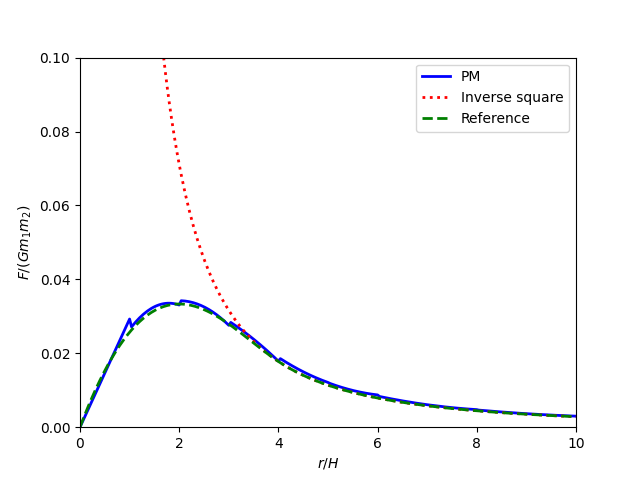
\includegraphics[scale=0.6]{img/optimal-green-force-4.png}
    \caption{Magnitude of the force between two masses.
        The mesh approximation to the reference force was calculated using the PM method with TSC assignment scheme, two-point finite difference, and the Green's function optimal for the $S_1$ shape with diameter $a=4H$.
        The force resultant from the universal law of gravitation is also shown.}
    \label{fig:reference-force-approx}
\end{figure}
As can be seen in the figure, the PM force closely follows the reference force.
Moreover, for $r>a$, the reference force is identical to the inverse-square force.
It is also worth noting that the reference force (and its mesh approximation) approximate the inverse-square force accurately for $r$ slightly smaller than $a$.
For this reason $r_e$, the \textit{cutoff radius} designating the boundary of the region handled by the direct summation, can be chosen to be smaller than $a$ (e.g. $r_e = 0.7a$).
This can have noticeable positive impact on performance.

\subsection{Identifying close pairs of particles}
In the \PThreeM{} method, in addition to the mesh used in the PM algorithm (the "potential mesh"), a second mesh (the \textit{chaining mesh}) is used.
The chaining mesh is sparser compared to the potential mesh and its sole purpose is to partition the space into cells so that particles "close" to the ones in a given cell can be found efficiently.
In this context, two particles are considered to be lying close to one another if their separation is less than the cutoff radius.

The number of chaining mesh cells in a single dimension is given by $M_i = \lfloor L_i / r_e \rfloor$, where $L_i$ is the side length of the computational box ($i=1,2,3$).
This implies that the side length of a chaining mesh cell is $HC_i = L_i / M_i \geq r_e$.
Thus, for every particle $i$ in a given cell $\mathbf{p}$, it is sufficient to search through the immediate neighborhood of $\mathbf{p}$ to find all the particles within the cutoff radius from $i$.

The chaining mesh can be implemented as a \textit{head-of-chain} (HOC) array, depicted in \autoref{fig:hoc}.
\begin{figure}[htp]
    \centering
    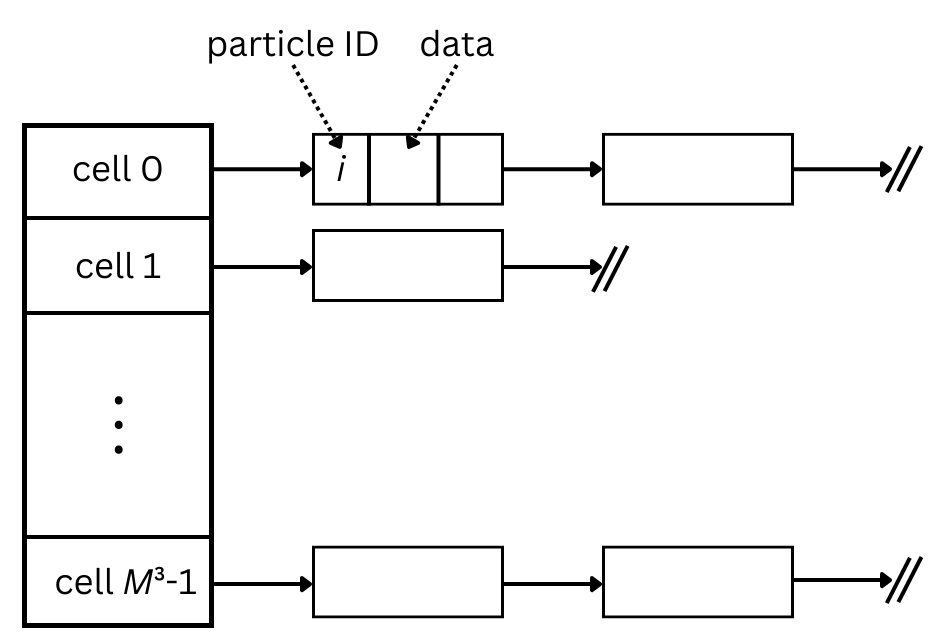
\includegraphics[scale=0.25]{img/hoc.png}
    \caption{Head-of-chain data structure used for mapping particles to their parent cells in the chaining mesh.
        Here $M_1=M_2=M_3 = M$.}
    \label{fig:hoc}
\end{figure}
The basic version of the HOC array is very cheap to build with the whole process being linear in the number of particles.
Hence, the array can be constructed anew at each time-step.
Additional computational savings can be made by preallocating a memory pool large enough to store $N$ nodes of the linked lists and using it for initializing the HOC array.
Another noteworthy possible optimization is to sort the individual linked lists by the value of a certain particle coordinate, say the $y$ coordinate.
This allows for an early return from the direct summation loop on the condition that $|y_i - y_j| > r_e$ while particle $i$ is sweeping through a cell containing particles $j$.

\subsection{Short-range correction}
The short-range correction, which takes place immediately after the mesh forces are found using the PM method, is at the heart of the \PThreeM{} algorithm.
Since it is quadratic in the number of particles in each neighborhood, it is imperative that further optimizations be put in place.

By the Newton's 3rd law, $\mathbf{f}^\text{SR}_{ji} = -\mathbf{f}^\text{SR}_{ij}$, which allows us to do the calculation of the short-range inter-particle force for any pair $(i, j)$ of particles only once, leading to the reduction of the total running time by half.
In practice, the particle $i$ will update its own total short-range force $\mathbf{F}^\text{SR}_i$ as well as the total short-range force $\mathbf{F}^\text{SR}_j$ of its neighbor $j$.
In order to avoid double-counting, the particle $i$ residing in cell $\mathbf{q}$ has to look for its neighbors in a subset $\mathcal{N}$ of the immediate neighborhood of $\mathbf{q}$.
More specifically, define
\begin{equation*}
    \mathcal{N}(\mathbf{q} = (q_1, q_2, q_3)) = \{(q_1+t, q_2-1,q_3+s), (q_1+s, q_2, q_3-1), (q_1-1,q_2,q_3) \;|\; s,t = -1,0,1 \}.
\end{equation*}
Thus $|\mathcal{N}| = 13$, which is half of the size of the immediate neighborhood.

The short-range correction part of the \PThreeM{} method is shown in \autoref{alg:short-range-correction}.
\begin{algorithm}
    \caption{Short-range correction}\label{alg:short-range-correction}
    \begin{algorithmic}
        \ForAll {chaining cell $\mathbf{q}$}
        \ForAll {$\mathbf{q}_n \in \mathcal{N}(\mathbf{q}) \cup \{\mathbf{q}\}$}
        \ForAll {$i \in \text{HOC}(\mathbf{q})$}
        \ForAll {$j \in \text{HOC}(\mathbf{q}_n)$}
        \If {$|y_i - y_j| > r_e$}
        \Break
        \EndIf
        \State \Call{UpdateShortRange}{$i$, $j$, $\mathbf{q}$, $\mathbf{q}_n$}
        \EndFor
        \EndFor
        \EndFor
        \EndFor
    \end{algorithmic}
\end{algorithm}
The \textsc{UpdateShortRange} procedure is defined in \autoref{alg:update-short-range-forces}.
\begin{algorithm}
    \caption{Updating short-range forces}\label{alg:update-short-range-forces}
    \begin{algorithmic}[1]
        \Procedure{UpdateShortRange}{$i$, $j$, $\mathbf{q}$, $\mathbf{q}_n$}
        \If {$i = j$}
        \Return
        \EndIf
        \State $\mathbf{r}_{ij} \gets \mathbf{r}_i - \mathbf{r}_j$
        \If {$|\mathbf{r}_{ij}|^2 > r_e^2$}
        \Return
        \EndIf
        \State $r_{ij} \gets |\mathbf{r}_{ij}|$
        \State $\hat{\mathbf{r}}_{ij} \gets \mathbf{r}_{ij} / r_{ij}$
        \State $\mathbf{R}_{ij} \gets -m_i m_j R(r_{ij}) \hat{\mathbf{r}}_{ij}$
        \State $\mathbf{f}^\text{tot} \gets -G m_i m_j / r_{ij}^2 \hat{\mathbf{r}}_{ij}$
        \State $\mathbf{f}^\text{SR}_{ij} \gets \mathbf{f}^\text{tot} - \mathbf{R}_{ij}$
        \State $\mathbf{f}^\text{SR}_{ji} \gets -\mathbf{f}^\text{SR}_{ij}$
        \State $\mathbf{F}^\text{SR}_i \gets \mathbf{F}^\text{SR}_i + \mathbf{f}^\text{SR}_{ij}$
        \If {$\mathbf{q}_n \neq \mathbf{q}$} \Comment{Avoid double-counting in the parent cell}
        \State $\mathbf{F}^\text{SR}_j \gets \mathbf{F}^\text{SR}_j + \mathbf{f}^\text{SR}_{ji}$
        \EndIf
        \EndProcedure
    \end{algorithmic}
\end{algorithm}
As suggested in \cite{Hockney1988}, the computational burden of operations in lines 5-8 in \autoref{alg:update-short-range-forces} can be greatly reduced by storing the values of $f^{SR}(r) / r$ in a lookup table $T$ at uniform intervals $\Delta^2$ of $[0, r_e^2]$ and interpolating.
The schematic depiction of the interpolation is shown in \autoref{fig:sr-force-val-interpolation}.
\begin{figure}[htp]
    \centering
    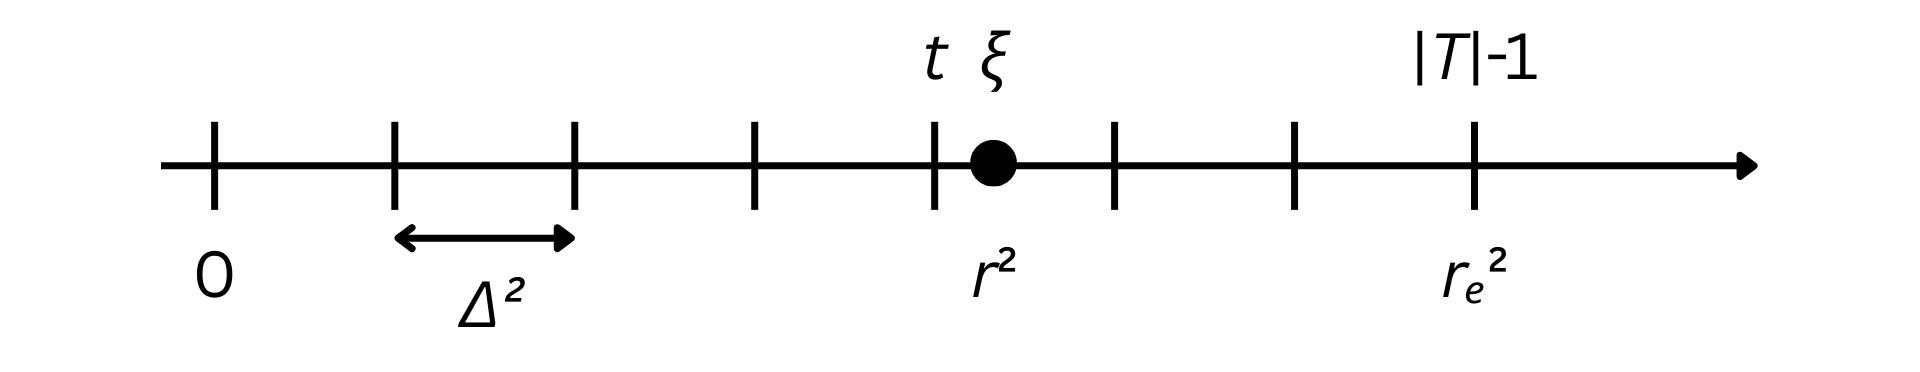
\includegraphics[scale=0.2]{img/interpolation.png}
    \caption{Interpolation of short-range force values.}
    \label{fig:sr-force-val-interpolation}
\end{figure}
If we define $\xi = r^2 / \Delta^2$ and $t=\lfloor \xi \rfloor$, then
\begin{equation*}
    \frac{f^\text{SR}(r)}{r} \approx T[t](1 - (\xi - t)) + F[t+1](\xi - t)
    = T[t] + (\xi - t) (T[t+1] - T[t]).
\end{equation*}
The value $\mathbf{f}^\text{SR}_{ij}$ can then be obtained by multiplying the interpolated quantity $f^\text{SR}(r_{ij})/r_{ij}$ by $G m_i m_j \mathbf{r}_{ij}$, completely eliminating the use of the square root operations and reducing the total number of flouting-point operations to just four.

The procedure outlined in\autoref{alg:short-range-correction} can be parallelized by splitting the work done in the outmost loop between some number of threads.
In doing so, extra care has to be taken to avoid data races.
A thread $t$ that is currently processing cell $\mathbf{p}$ and its neighbors (we say that $t$ is \textit{assigned} to $\mathbf{p}$) may "clash" with a different thread processing a nearby cell $\mathbf{q}$ (because possibly $\mathbf{p} \in \mathcal{N}(\mathbf{q})$).
However, by construction of the set $\mathcal{N}$, it is possible to split the short-range force into 14 parts, each of which is accessed by only one thread.
For example, consider a particle $i$ in cell $\mathbf{p} = (p_1, p_2, p_3)$ (in other words, $\mathbf{p}$ is the parent cell of $i$).
If thread $t$ is currently assigned to this cell, $t$ will update the part of $\mathbf{F}^\text{SR}_i$ corresponding to updates of $i$ coming from within the same cell as the parent cell of $i$.
Possibly at the same time, thread $t'$ assigned to cell $\mathbf{q} = (p_1+1, p_2, p_3)$ will update a different part of $\mathbf{F}^\text{SR}_i$, i.e. the part corresponding to updates of $i$ coming from the cell "to the right" of the parent cell of $i$.
Since only one thread is responsible for updates coming "from the the right," no data races can occur.